% ======================================================================
\section{Why the problem is hard for today's models}\label{sec:hard}

A reader may expect that modern models solve this task directly: a sound tagger hears the siren, a vision model
says whether an ambulance is on screen, an image model draws it. This section explains, step by step, why that does
not happen. ``Hard'' here means hard for open models of up to about 70\,GB, chained without training; a much larger
vision model (Qwen3-VL-235B) was not tested, and fine-tuning was outside the design. Each subsection states what one
might expect, what actually happens, and the evidence. Table~\ref{tab:naive} summarises the argument and
Table~\ref{tab:scale} the size of the search behind it.

\begin{table}[htbp]
\centering\small
\caption{The obvious ready-made chain, step by step: what goes wrong, and what the final system does instead.}
\label{tab:naive}
\begin{tabular}{L{1.5cm}L{2.6cm}L{5.0cm}L{4.9cm}}
\toprule
Step & Ready-made choice & What goes wrong (evidence) & What the final system does \\
\midrule
Hear & one sound tagger & quiet sounds under speech or music never become candidates; under 40\,\% of raw detections
are real (Section~\ref{sec:hard-hear}) & two complementary detectors, with every weak candidate checked \\
Confirm & ask an audio-language model & a sound one listener names is real 37\,\% of the time
(Figure~\ref{fig:listeners}) & a weak sound needs a witness: DASM, both listeners, or one listener plus the scene \\
See & ask a vision-language model ``is it visible?'' & presence is taken for production (31 of 36 audited errors);
AUROC 0.647; answers follow the question's form & three questions per 5-s stretch, asked in both orders; silenced only if
every stretch is visible \\
Draw & audio-to-image model & draws the whole scene, including what is on screen & label-guarded text prompt;
the picture is checked and redrawn up to five times \\
Score & model judge & circular or at chance on visibility (Section~\ref{sec:hard-measure}) & per-sound human labels
and a viewer cost \\
\midrule
All & draw every detected sound & 62 wrong for 26 right on the test set; no better than showing nothing &
final system: 24 wrong for 24 right; cheaper than both baselines \\
\bottomrule
\end{tabular}
\end{table}

\begin{table}[htbp]
\centering\small
\caption{Scale of the study behind the final system (details in Appendix~\ref{app:history}).}
\label{tab:scale}
\begin{tabular}{L{5.2cm}L{9.0cm}}
\toprule
What & How much \\
\midrule
Open models evaluated & more than 30: 14 sound detectors and taggers (e.g.\ BEATs, FlexSED, PANNs, AST, EAT, Dasheng,
CLAP, FLAM, DASM, FineLAP), 6 audio-language listeners, 2 source separators, 8 vision models and tools (CLIP, two
Qwen vision-language models, OWLv2, SAM 3, SigLIP, a sound localiser, Synchformer), 3 image generators (SDXL, FLUX.1,
Qwen-Image), and several model judges \\
Pre-registered rounds & 66 rounds, each with its rule and pass bar written before the run \\
Full-pipeline variants scored & more than 150, plus about 90 component screens \\
Human labels & 308 timed sounds in 159 clips, each marked visible or not and rated for importance \\
Screening data & 415 AudioSet-Strong clips with timed labels for audio-only rules \\
\bottomrule
\end{tabular}
\end{table}

\subsection{Hearing the sound at all}\label{sec:hard-hear}
\emph{Expected:} a modern tagger hears a hammer or a door. \emph{Actually:} under speech or music it often does not.
The tagger's own score for \emph{Speech} or \emph{Music} is higher than for the quiet sound, so the sound never becomes
a candidate. In a ceiling analysis of an earlier version (each later step is made perfect using the labels, to see what the
detectors alone allow), even with every later stage made perfect about one needed
sound in five (12 of 55) stayed missed, because no model heard it clearly (Figure~\ref{fig:ceiling}; numbers in
Section~\ref{sec:ceiling}). Removing the speech first with a source separation model made it worse: on DCASE data (a
public challenge set of everyday sound events), the share of sounds found under speech
fell from 9.5\,\% to 4.8\,\%, because the
detectors were never trained on separated audio.


\begin{figure}[htbp]
\centering
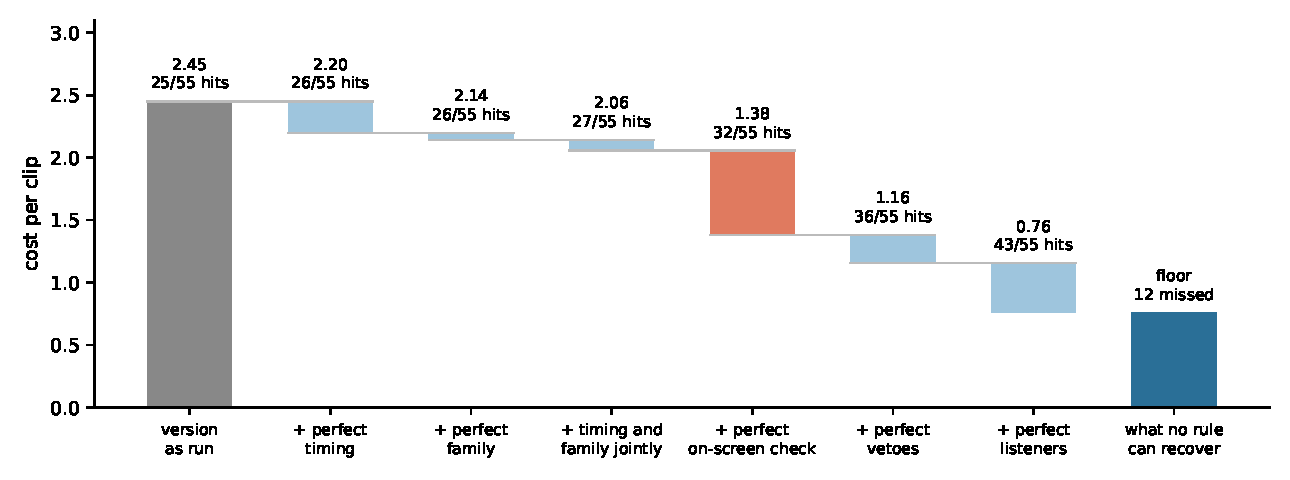
\includegraphics[width=\linewidth]{figures/ceiling_waterfall.pdf}
\caption{Ceiling analysis on a slightly older version of the system (development set, 55 needed sounds). Each bar makes
one more stage perfect, using the labels, on the same detections. The largest single step is the on-screen check. Even
with every stage perfect, 12 needed sounds remain missed (right): the detectors never hear them clearly enough.}
\label{fig:ceiling}
\end{figure}

\subsection{Knowing whether a weak detection is real}
\emph{Expected:} an audio-language model can confirm ``is there a siren?''. \emph{Actually:} its answers are only
weak evidence. On the screening set, a weak detection that neither listener names is a real sound 22\,\% of the time,
one named by one listener 37\,\%, and one named by both 62\,\% (Figure~\ref{fig:listeners}; AudioSet labels are
incomplete, so these shares are lower bounds, and the ordering, not the level, is the evidence). Raw detections are right
under 40\,\% of the time. A full chain of listener, timing and DASM checks reaches 80\,\%, but only for the few sounds
that survive the chain. Every way to add more
sounds found real ones but paid two to five wrong pictures per new hit. The best such rule found two more hits than the
final system on the development set, at about five extra wrong pictures each (31 hits and 26 wrong, against 29 and 15),
so it failed the development rule; its test result, reported only, was no better (25 hits and 35 wrong, against 24 and
24). Nothing later in the chain can tell a
right off-screen name from a wrong one.


\begin{figure}[htbp]
\centering
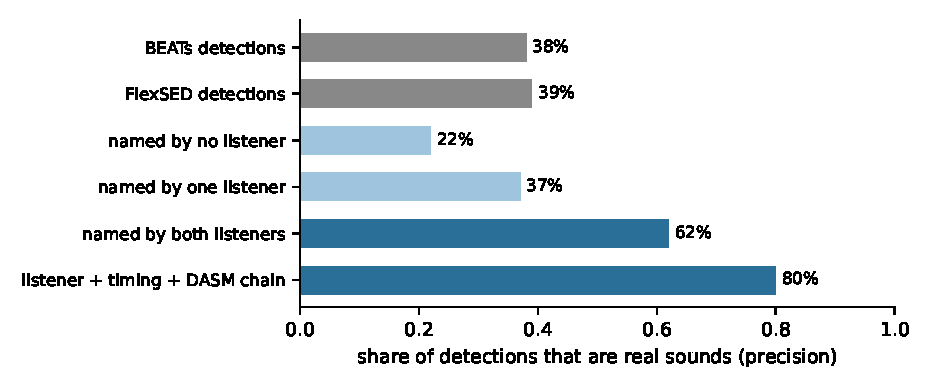
\includegraphics[width=0.78\linewidth]{figures/listener_agreement.pdf}
\caption{Share of detections that are real sounds, on the screening set (415 AudioSet-Strong clips with timed labels).
Raw detections are right less than 40\,\% of the time; agreement between models helps, but a sound only one listener
names is right just over a third of the time. The last bar is the audio chain of a rejected idea (Appendix~\ref{app:history}),
shown for reference.}
\label{fig:listeners}
\end{figure}

\subsection{``It is there'' is not ``it is making the sound now''}
\emph{Expected:} a vision-language model can answer ``is this bell ringing?''. \emph{Actually:} it answers ``is there a
bell?''. A church tower on screen silences a bell heard off screen; perched birds are taken as the source of a call
made elsewhere. In a hand audit of 36 stretches that the gate wrongly silenced, 31 showed either the named object not making the
sound, or a similar object (Section~\ref{sec:presence}). The opposite failure is also large: asked to name the
source, the model answers ``nothing'' on 42\,\% of the stretches the labels call visible or obvious (a hand, the footsteps of the
person holding the camera). The problem is old: an early image-text matching check (CLIP) was right only about half the time. Moving from a
7-billion- to a 27-billion-parameter vision model raised balanced accuracy (the mean of the success rates on visible
and on needed sounds) only from 0.61 to 0.62.

\subsection{Every fix to the on-screen check trades one for one}
\emph{Expected:} adding an object detector, a segmentation model, a crop of the source, a model of audio-visual
synchrony or a sound-localisation model should help. \emph{Actually:} each one silenced more on-screen sounds only by
silencing about as many needed ones (Figure~\ref{fig:gate}). Removing two wrong pictures saves $2\times2 = 4$ cost units;
losing one needed sound costs 4: no gain. Localisation models also react to off-screen and silent audio, so they answer
\emph{where} a sound comes from, not \emph{whether} its source is visible.


\begin{figure}[htbp]
\centering
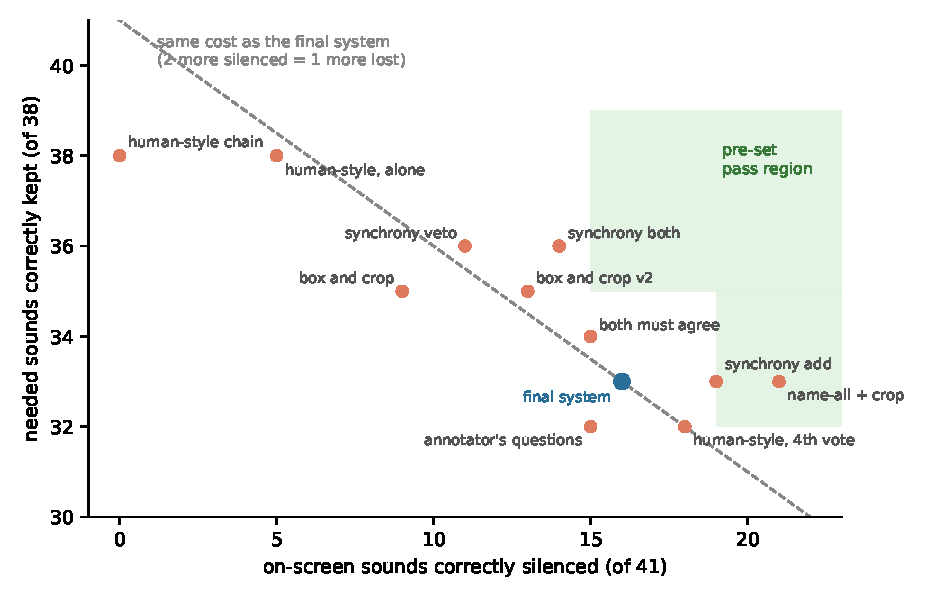
\includegraphics[width=0.8\linewidth]{figures/gate_tradeoff.pdf}
\caption{Every variant of the on-screen check that was tried, scored on the subset of development sounds that reach
the check and whose stretches the author labelled (41 on-screen sounds, 38 needed sounds). The dashed line has the same cost as the final system: silencing two more
on-screen sounds is worth losing one needed sound. All variants lie near this line, and none reached the pass region
fixed before the tests. Labels name the extra tool tried: an object box, a crop around the named object, an audio-visual
synchrony model, a longer human-style question chain, or a fourth vote.}
\label{fig:gate}
\end{figure}

\subsection{Answers follow the shape of the question}
\emph{Expected:} a clear question gets a clear answer. \emph{Actually:} given options (a) and (b), the 27B model picks
(a) 88\,\% of the time in one test; asked yes/no, it leans to ``no''; asked for free text, its answer can be cut off.
Two workarounds are used. The scene check reads the model's preference for ``yes'' over ``no'' as a number
instead of reading its words (minus the same for the opposite question); the on-screen check asks its a/b question in
both orders and abstains if the answers disagree. This removes the habits but exposes the real weakness: when the
on-screen check's own a/b question is read the same way, as a score, it separates visible from needed sounds on the
labelled development stretches with an AUROC of only 0.647 (the chance that a random visible stretch scores higher
than a random needed one; 0.5 is a coin flip, 1 is perfect). The habits were hiding a weakness, not causing it.

\subsection{Drawing one unseen source, not a scene}
\emph{Expected:} an audio-to-image model can draw what is heard. \emph{Actually:} such models draw the whole soundtrack
as a scene and cannot be told to leave out the dog that is already on screen. The system therefore draws from the label
with a guarded text prompt -- and even then a picture was named right at a glance in only 26 of 54 tries
(Section~\ref{sec:pictures}). A richer prompt reached 32 of 54 but invented objects (a thud drawn as a door).

\subsection{Measuring success is hard too}\label{sec:hard-measure}
The proposal planned an automatic score: one model describes the output video, another writes a reference of what
a viewer should learn, and a third model (the judge) compares the two. \emph{Expected:} a model judge can score the
output. \emph{Actually:} a reference written by the system's own models
rewards the system; one written by independent models agreed with the human ``nothing is missing'' label on 55 of
100 clips, which is chance; and the best judge scored a picture and a text tag the same (Appendix~\ref{app:judge}).
Existing labels do not help either: AudioSet names only a few sounds per clip, so on an AudioSet calibration set an
earlier version of the system looked worse than showing nothing (1.650 against 0.986 per clip), although on full
labels it is clearly better. Even full human
labels miss some sounds: about 1 in 6 ``wrong'' pictures is a real off-screen sound, and 14 borderline development
sounds sit one judgement away from the other class.

\subsection{The data is rare}
Clips in which an ambient sound is heard but its source is not seen are uncommon in public video. Four different
sourcing routes all yielded only 15--20\,\% usable clips, which is why the benchmark has 159 evaluation clips rather than
the planned 300, and why every comparison has wide intervals.

\subsection{What today's models are missing}\label{sec:missing}
The failures above point to six capabilities that current open models lack. Each one is a direction in which a better
model, not a better rule, is needed.
\begin{enumerate}
  \item \textbf{Hearing a quiet event under speech or music.} Taggers are trained to name the dominant sound of a clip, so a
        door under a conversation loses to \emph{Speech}. Separating the speech first does not help, because the
        detectors have never heard separated audio (Section~\ref{sec:hard-hear}). What is missing is detection trained on
        mixtures in which the event of interest is the quiet one.
  \item \textbf{Knowing when not to say yes.} A listener asked ``is there a siren?'' tends to agree, and a sound one listener
        names is real only 37\,\% of the time. What is missing is a calibrated answer: a confidence that means the same
        thing from one question to the next, or the option to answer ``not sure''.
  \item \textbf{Linking an object to the sound it is making now.} Vision-language models answer ``is there a bell?'' when asked
        ``is the bell ringing?'' (31 of 36 audited gate errors). They see objects, not actions that produce sound, and
        they do not use the audio. What is missing is audio-visual grounding of \emph{production}: does this object's
        motion match this sound at this moment?
  \item \textbf{Saying that a source is off screen.} Sound-source localisation models always point somewhere in the
        frame, even for off-screen or silent audio~\cite{juanola2025critical}. What is missing is an explicit
        ``not in the frame'' answer, which is exactly the decision this task needs.
  \item \textbf{Drawing one source and leaving out the rest.} Audio-to-image models draw the whole soundtrack as one scene.
        What is missing is a generator that takes a negative condition from the video (``a dog, but not the dog that is
        already visible'') and draws one clear object for a glance.
  \item \textbf{Judging per sound.} Model judges score a whole clip and cannot tell whether a picture matches a specific
        sound at a specific time, or whether that sound was visible. What is missing is an evaluator that works at the
        level of single timed sounds; until then, human per-sound labels are required.
\end{enumerate}
The system in this report works around each gap with rules: two detectors, independent witnesses, a three-question
vote, guarded prompts with a check-and-redraw loop, and human labels. A model that closed any one of these gaps would
remove a whole family of rules.
